\section{第二章\quad 传输线理论}

\begin{frame}{传输线理论}
 \begin{itemize}
  \item \textbf{传输线理论,一维分布参数电路理论,微波电路设计和计算的理论基础。}
  \item \textbf{传输线理论,电路理论与场的理论之间起着桥梁的作用。}
 \end{itemize}
\end{frame}

\subsection{传输线方程}
\begin{frame}{传输线方程}
 \begin{enumerate}
  \item 传输线的电路模型
 \end{enumerate}
 \centering
 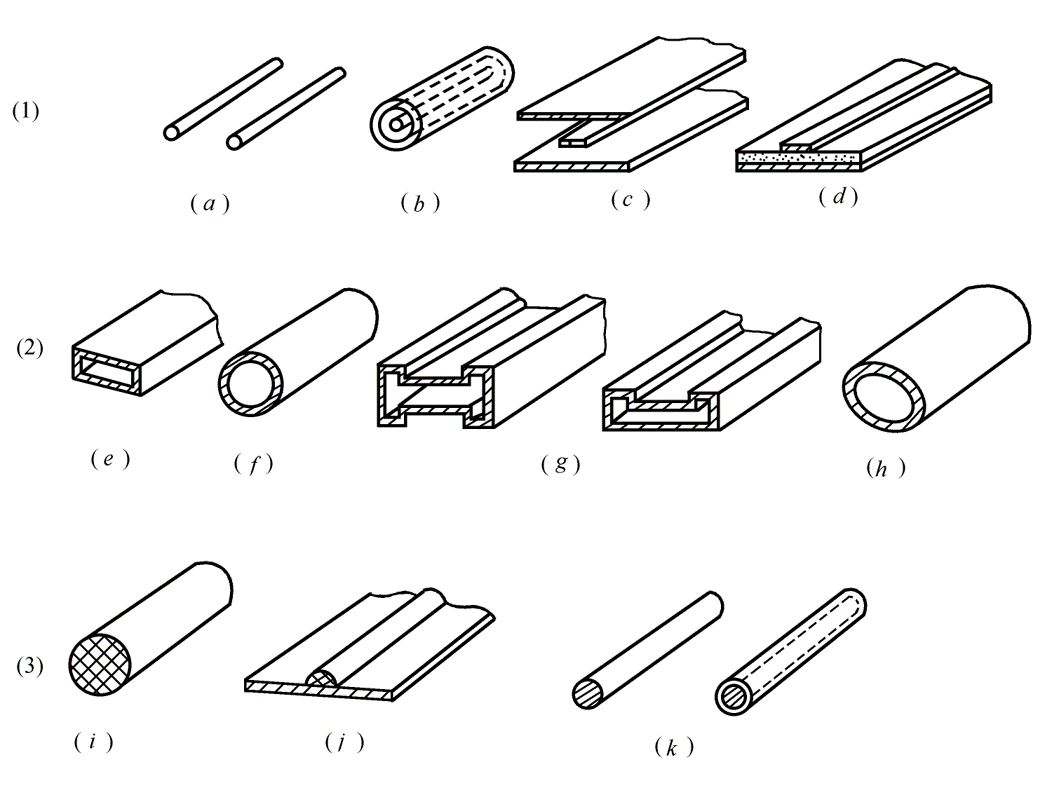
\includegraphics[width=9cm]{guidesystem.png}
 \saveenum
\end{frame}

\begin{frame}{传输线方程}
 \textbf{传输线}是以TEM导模的方式传送电磁波能量或信号的导行系统,其横向尺寸远小于其上工作波长。\\
 \textbf{传输线}有\textbf{长线}和\textbf{短线}之分。所谓长线是指传输线的几何长度与线上传输电磁波的波长比值(电长度)可相比拟,反之称为短线。\\
 \begin{align*}
  \text{长线}\Longrightarrow\text{分布参数电路} \\
  \text{短线}\Longrightarrow\text{集中参数电路} \\
  \text{分界线:}\widefbox{$l/\lambda\geq 0.05$}
 \end{align*}
 当频率提高到微波波段时,这些分布效应不可忽略,所以微波传输线是一种\textbf{分布参数电路}。这导致传输线上的电压和电流是随时间和空间位置而变化的二元函数。
\end{frame}

\begin{frame}{传输线方程}
 根据传输线上的分布参数是否均匀分布,可将其分为均匀传输线和不均匀传输线。我们可以把均匀传输线分割成许多小的微元段$dz(dz<<\lambda)$,这样每个微元段可以看作集中参数电路,用一个$\Gamma$型网络来等效。于是整个传输线可等效成无穷多个$\Gamma$型网络的级联。\\
 \centering
 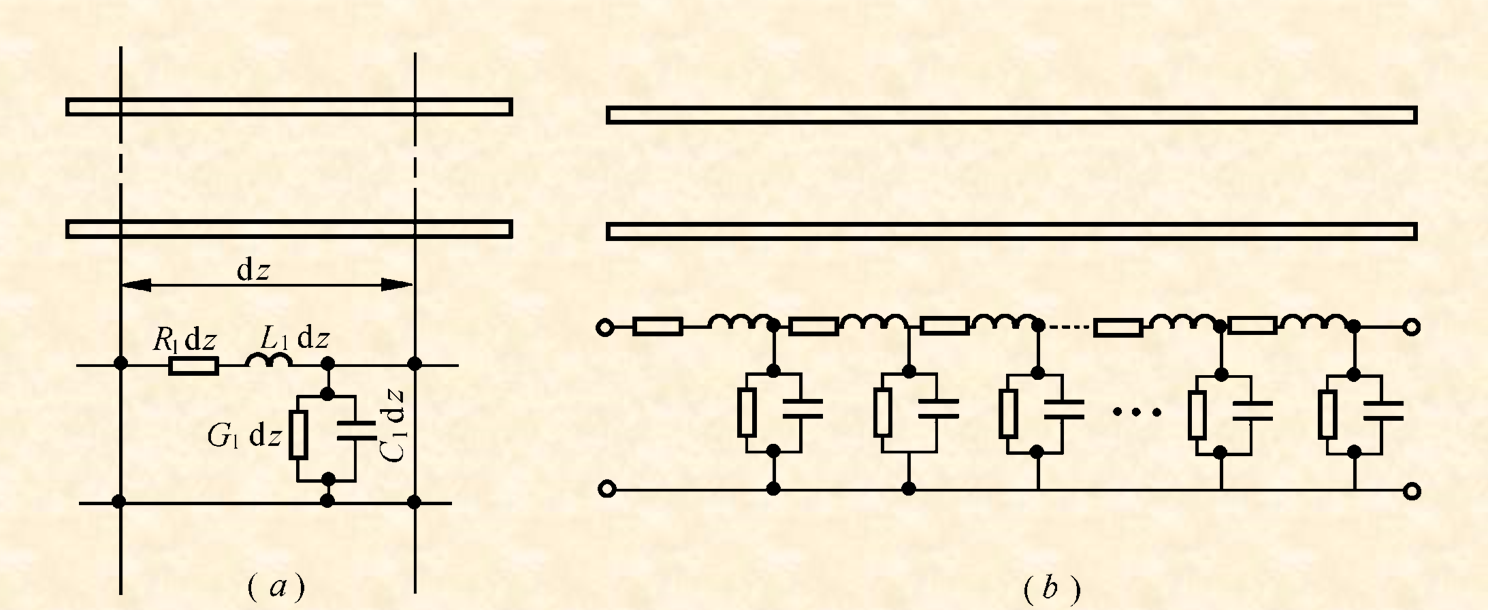
\includegraphics[width=9cm]{transmissionline1.png}
\end{frame}

\begin{frame}{传输线方程}
 双导线、同轴线和平行线传输线的分布参数\\
 \centering
 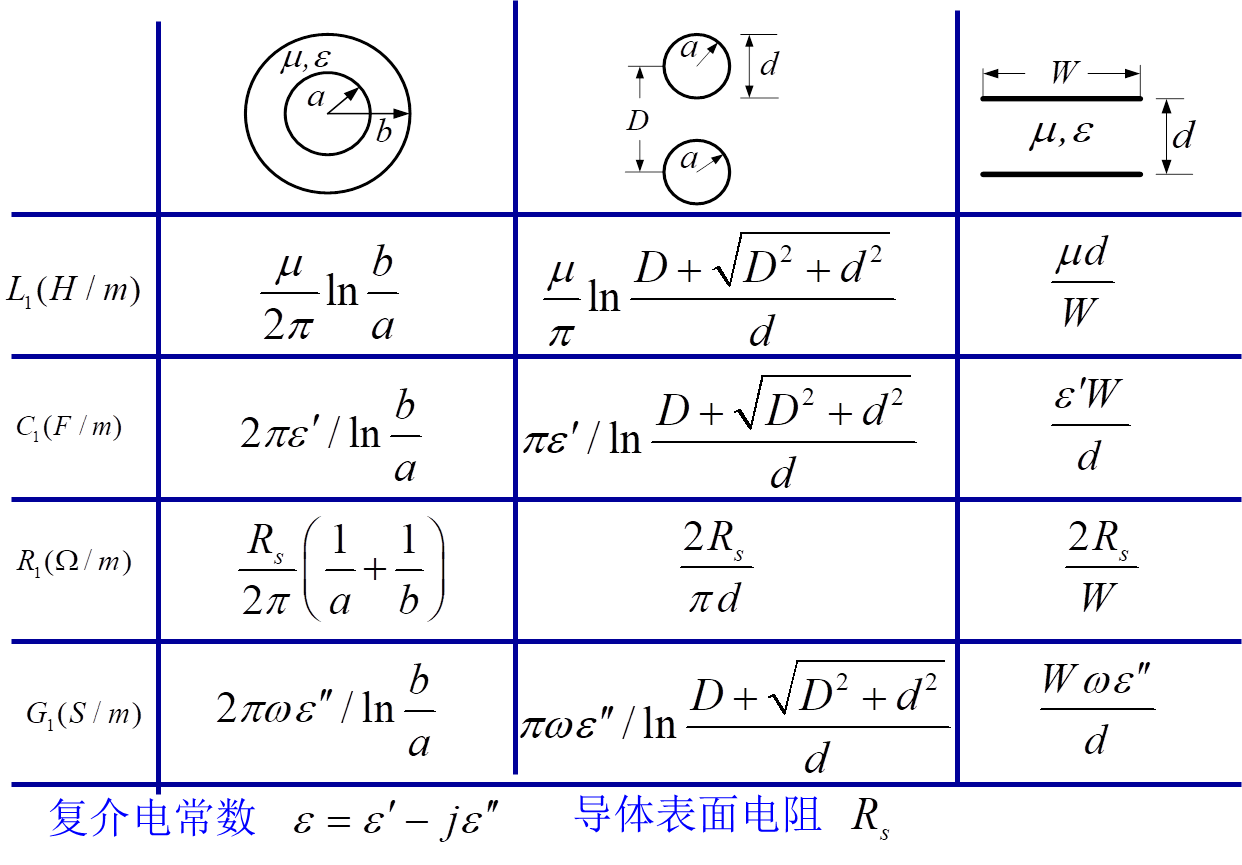
\includegraphics[width=9cm]{tmlineparas.png}
\end{frame}

\begin{frame}{传输线方程}
 \begin{enumerate}
  \resume
  \item 传输线方程\\
        \begin{itemize}
         \item 一般传输线方程或电报方程\\
               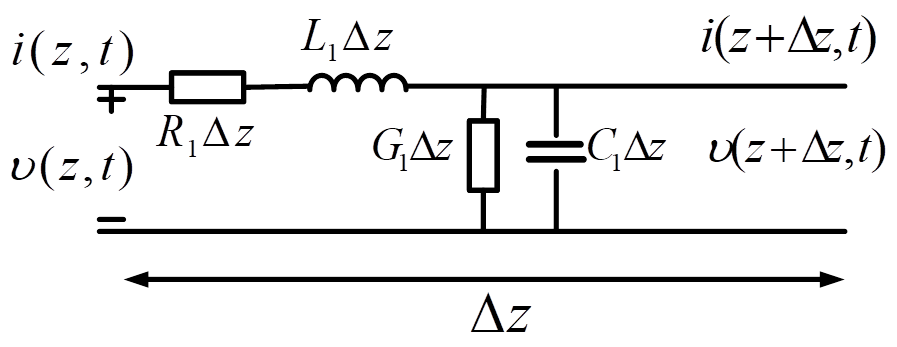
\includegraphics[width=6cm]{transmissionline2.png}
        \end{itemize}
        \saveenum
 \end{enumerate}
 \flushleft
 \fbox{$ v(z+\Delta z,t)=v(z,t)+\frac{\partial v(z,t)}{\partial z}\Delta z $}
 \flushright
 \fbox{$ i(z+\Delta z,t)=i(z,t)+\frac{\partial i(z,t)}{\partial z}\Delta z $}\\
 \begin{align*}
   f(x)=f(x_{0})+f^{'}(x_{0})(x-x_{0})  +\frac{f^{''}(x_{0})}{2!}(x-x_{0})^{2}+\ldots\\
   +\frac{f^{n}(x_{0})}{n!}(x-x_{0})^{n}+R_{n}(x)
 \end{align*}
\end{frame}

\begin{frame}{传输线方程}
  \centering
  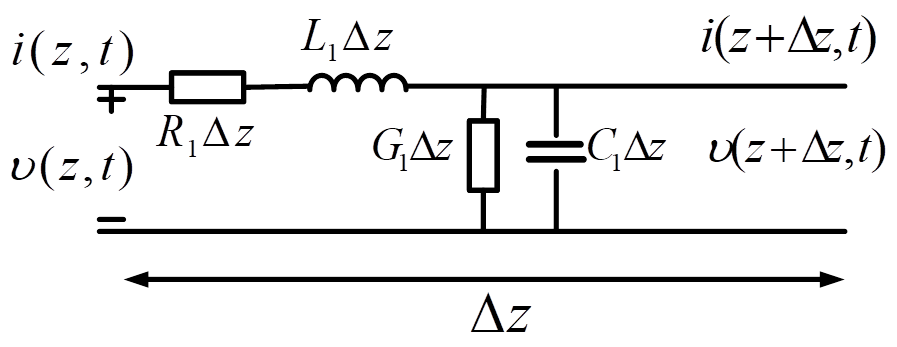
\includegraphics[width=7cm]{transmissionline2.png}
  \flushleft
  线元$\Delta z$上的电压、电流的变化为:
  \begin{empheq}[box=\widefbox]{align*}
    v(z,t)-v(z+\Delta z,t)=-\frac{\partial v(z,t)}{\partial z}\Delta z\\
    i(z,t)-i(z+\Delta z,t)=-\frac{\partial i(z,t)}{\partial z}\Delta z
  \end{empheq}
\end{frame}

\begin{frame}{传输线方程}
  \centering
  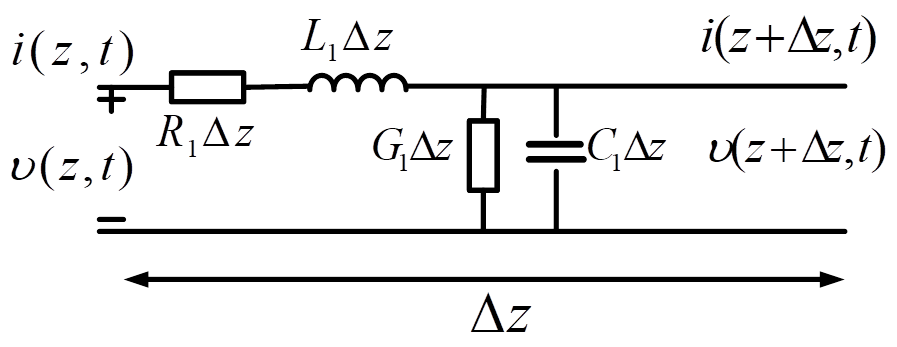
\includegraphics[width=7cm]{transmissionline2.png}
  \flushleft
  线元$\Delta z$上应用基尔霍夫定律,可得:
  \begin{empheq}[box=\widefbox]{align*}
    -\frac{\partial v(z,t)}{\partial z}\Delta z=R_{1}\Delta z\cdot i(z,t)+L_{1}\Delta z\cdot\frac{\partial i(z,t)}{\partial t}\\
    -\frac{\partial i(z,t)}{\partial z}\Delta z=G_{1}\Delta z\cdot v(z,t)+C_{1}\Delta z\cdot\frac{\partial v(z,t)}{\partial t}
  \end{empheq}
\end{frame}

\begin{frame}{传输线方程}
  \begin{empheq}[box=\widefbox]{align*}
    -\frac{\partial v(z,t)}{\partial z}\Delta z=R_{1}\Delta z\cdot i(z,t)+L_{1}\Delta z\cdot\frac{\partial i(z,t)}{\partial t}\\
    -\frac{\partial i(z,t)}{\partial z}\Delta z=G_{1}\Delta z\cdot v(z,t)+C_{1}\Delta z\cdot\frac{\partial v(z,t)}{\partial t}
  \end{empheq}
  \flushleft
  令$\Delta z \rightarrow 0$
  \begin{empheq}[box=\widefbox]{align*}
    \frac{\partial v(z,t)}{\partial z}=-R_{1}\cdot i(z,t)-L_{1}\cdot\frac{\partial i(z,t)}{\partial t}\\
    \frac{\partial i(z,t)}{\partial z}=-G_{1}\cdot v(z,t)-C_{1}\cdot\frac{\partial v(z,t)}{\partial t}
  \end{empheq}
  \centering
  \textbf{一般传输线方程、电报方程}
\end{frame}

\begin{comment}
\newcommand{\mtikzmark}[1]{\tikz[overlay,remember picture]\node(#1){};}
\tikzset{mylabel/.style={align=center,fill=blue!10,font=\footnotesize}}
%\mytlabel[options]{start.mark}{end.mark}{text}
\newcommand\mytlabel[4][]{%
 \tikz[overlay,remember picture]
 {\draw[->]([yshift=-10pt]#2.north) -- node[mylabel,#1]{#4}([yshift=6pt]#3.north);}
}
\end{comment}

\begin{frame}{传输线方程}
  \begin{itemize}
    \item 时谐均匀传输线方程
  \end{itemize}
  \begin{empheq}[box=\widefbox]{align*}
    \frac{\partial v(z,t)}{\partial z}=-R_{1}\cdot i(z,t)-L_{1}\cdot\frac{\partial i(z,t)}{\partial t}\\
    \frac{\partial i(z,t)}{\partial z}=-G_{1}\cdot v(z,t)-C_{1}\cdot\frac{\partial v(z,t)}{\partial t}
  \end{empheq}
  \begin{columns}
    \begin{column}{0.5\linewidth}
      \begin{empheq}[box=\widefbox]{align*}
        v(z,t)=Re\left[V(z)e^{j\omega t}\right]\\
        i(z,t)=Re\left[I(z)e^{j\omega t}\right]
      \end{empheq}
    \end{column}
    \begin{column}{0.5\linewidth}
      分布参数:$R_{1}$,$L_{1}$,$C_{1}$,$G_{1}$不随位置变化
    \end{column}
  \end{columns}
\end{frame}

\begin{frame}{传输线方程}
  \begin{empheq}[box=\widefbox]{align*}
    \frac{dV(z)}{dz}=-(R_{1}+j\omega L_{1})I(z)=-Z_{1}I(z)\\
    Z_{1}=R_{1}+j\omega L_{1} \text{:单位长度串联阻抗}
  \end{empheq}
  \begin{empheq}[box=\widefbox]{align*}
    \frac{dI(z)}{dz}=-(G_{1}+j\omega C_{1})V(z)=-Y_{1}V(z)\\
    Y_{1}=G_{1}+j\omega C_{1} \text{:单位长度并联导纳}
  \end{empheq}
  对$z$再微商
  \begin{align*}
    \frac{d^2}{dz^2}\left\{
    \begin{aligned}
      V(z)\\I(z)
    \end{aligned}
    \right\}-\gamma^2
    \left\{\begin{aligned}
      V(z)\\I(z)
    \end{aligned}\right\}=0
  \end{align*}
  \textbf{电压传播常数}:\fbox{$\gamma=\sqrt{Z_{1}Y_{1}}=\sqrt{(R_{1}+j\omega L_{1})(G_{1}+j\omega C_{1})}$}
\end{frame}

\begin{frame}{传输线方程}
  \begin{itemize}
    \item 时谐传输线方程电压、电流通解
  \end{itemize}
  电压:
  \begin{empheq}[box=\widefbox]{align*}
    V(z)=A_{1}e^{-\gamma z}+A_{2}e^{\gamma z}
  \end{empheq}
  电流:
  \begin{empheq}[box=\widefbox]{align*}
    I(z)=-\frac{1}{R_{1}+j\omega L_{1}}\frac{dV(z)}{dz}=\frac{1}{Z_{0}}(A_{1}e^{-\gamma z}-A_{2}e^{\gamma z})
  \end{empheq}
  $$\gamma=\sqrt{Z_{1}Y_{1}}=\sqrt{(R_{1}+j\omega L_{1})(G_{1}+j\omega C_{1})}$$
  \textbf{特性阻抗}:
  \begin{empheq}[box=\widefbox]{align*}
    Z_{0}=\sqrt{\frac{R_{1}+j\omega L_{1}}{G_{1}+j\omega C_{1}}}
  \end{empheq}
\end{frame}

\begin{frame}{传输线方程}
  \begin{itemize}
    \item 传输线方程的边界条件和解
  \end{itemize}
  \begin{columns}
    \begin{column}{0.35\linewidth}
      端接条件确定常数:\\
      终端条件\\
      始端条件\\
      信号源和负载条件
    \end{column}
    \begin{column}{0.65\linewidth}
      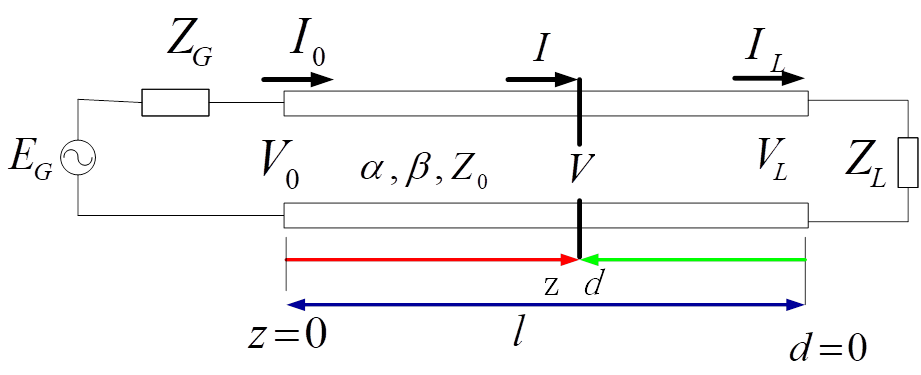
\includegraphics[width=6cm]{tmlineboundary.png}
    \end{column}
  \end{columns}
  \textbf{终端条件}解:
  \begin{columns}
    \begin{column}{0.5\linewidth}
      \begin{empheq}[box=\widefbox]{align*}
        V(z)=A_{1}e^{-\gamma z}+A_{2}e^{\gamma z}
      \end{empheq}
    \end{column}
    \begin{column}{0.5\linewidth}
      \begin{empheq}[box=\widefbox]{align*}
        I(z)=(A_{1}e^{-\gamma z}-A_{2}e^{\gamma z})/Z_{0}
      \end{empheq}
    \end{column}
  \end{columns}
  \begin{empheq}[box=\widefbox]{align*}
    V(l)=V_{L}=A_{1}e^{-\gamma l}+A_{2}e^{\gamma l}\\
    I(l)=I_{L}=\frac{1}{Z_{0}}(A_{1}e^{-\gamma l}-A_{2}e^{\gamma l})
  \end{empheq}
\end{frame}

\begin{frame}{传输线方程}
  \begin{empheq}[box=\widefbox]{align*}
    A_{1}=\frac{V_{L}+I_{L}Z_{0}}{2}e^{\gamma l},A_{2}=\frac{V_{L}-I_{L}Z_{0}}{2}e^{-\gamma l}
  \end{empheq}
  代入:
  \begin{columns}
    \begin{column}{0.45\linewidth}
      \begin{empheq}[box=\widefbox]{align*}
        V(z)=A_{1}e^{-\gamma z}+A_{2}e^{\gamma z}
      \end{empheq}
    \end{column}
    \begin{column}{0.45\linewidth}
      \begin{empheq}[box=\widefbox]{align*}
        I(z)=(A_{1}e^{-\gamma z}-A_{2}e^{\gamma z})/Z_{0}
      \end{empheq}
    \end{column}
  \end{columns}
  对于终端边界条件场合,我们常采用$d$(终端出发)坐标系$d$,换坐标\fbox{$d=l-z$}
  \begin{empheq}[box=\widefbox]{align*}
    V(d)=\frac{V_{L}+I_{L}Z_{0}}{2}e^{\gamma d}+\frac{V_{L}-I_{L}Z_{0}}{2}e^{-\gamma d}=V^{+}(d)+V^{-}(d)\\
    I(d)=\frac{V_{L}+I_{L}Z_{0}}{2Z_{0}}e^{\gamma d}-\frac{V_{L}-I_{L}Z_{0}}{2Z_{0}}e^{-\gamma d}=I^{+}(d)+I^{-}(d)
  \end{empheq}
\end{frame}

\begin{frame}{传输线方程}
  \begin{empheq}[box=\widefbox]{align*}
    V(d)=\frac{V_{L}+I_{L}Z_{0}}{2}e^{\gamma d}+\frac{V_{L}-I_{L}Z_{0}}{2}e^{-\gamma d}=V^{+}(d)+V^{-}(d)\\
    I(d)=\frac{V_{L}+I_{L}Z_{0}}{2Z_{0}}e^{\gamma d}-\frac{V_{L}-I_{L}Z_{0}}{2Z_{0}}e^{-\gamma d}=I^{+}(d)+I^{-}(d)
  \end{empheq}
  \begin{empheq}[box=\widefbox]{align*}
    V(d)=\frac{e^{\gamma d}+e^{-\gamma d}}{2}V_{L}+\frac{e^{\gamma d}-e^{-\gamma d}}{2}Z_{0}I_{L}\\
    I(d)=\frac{e^{\gamma d}+e^{-\gamma d}}{2}\frac{1}{Z_{0}}V_{L}+\frac{e^{\gamma d}-e^{-\gamma d}}{2}I_{L}
  \end{empheq}
  \begin{align*}
    \begin{bmatrix}
      V(d)\\I(d)
    \end{bmatrix}
    =
    \begin{bmatrix}
      ch\gamma d & Z_{0}sh\gamma d\\
      Z_{0}^{-1}sh\gamma d & ch\gamma d
    \end{bmatrix}
    \begin{bmatrix}
      V_{L}\\I_{L}
    \end{bmatrix}
  \end{align*}
\end{frame}

\begin{frame}{传输线方程}
  \textbf{始端条件解}:已知始端电压和电流$V_{0},I_{0}$ \\
  \fbox{$V(z)=A_{1}e^{-\gamma z}+A_{2}e^{\gamma z}$}
  \fbox{$I(z)=(A_{1}e^{-\gamma z}-A_{2}e^{\gamma z})/Z_{0}$}\\
  \begin{columns}
    \begin{column}{0.3\linewidth}
      \begin{align*}
        V_{0}=A_{1}+A_{2}\\
        I_{0}=(A_{1}-A_{2})/Z_{0}
      \end{align*}
    \end{column}
    \begin{column}{0.1\linewidth}
      \centering
      $ \longrightarrow $
    \end{column}
    \begin{column}{0.6\linewidth}
      \begin{empheq}[box=\fbox]{align*}
        A_{1}=\frac{V_{0}+I_{0}Z_{0}}{2}\quad A_{2}=\frac{V_{0}-I_{0}Z_{0}}{2}
      \end{empheq}
    \end{column}
  \end{columns}
  \begin{empheq}[box=\widefbox]{align*}
    V(z)=\frac{V_{0}+I_{0}Z_{0}}{2}e^{-\gamma z}+\frac{V_{0}-I_{0}Z_{0}}{2}e^{\gamma z}\\
    I(z)=\frac{V_{0}+I_{0}Z_{0}}{2Z_{0}}e^{-\gamma z}+\frac{V_{0}-I_{0}Z_{0}}{2Z_{0}}e^{\gamma z}
  \end{empheq}
  \begin{align*}
    \begin{bmatrix}
      V(d)\\I(d)
    \end{bmatrix}
    =
    \begin{bmatrix}
      ch\gamma z & -Z_{0}sh\gamma z\\
      -Z_{0}^{-1}sh\gamma z & ch\gamma z
    \end{bmatrix}
    \begin{bmatrix}
      V_{0}\\I_{0}
    \end{bmatrix}
  \end{align*}
\end{frame}

\begin{frame}{传输线方程}
  \textbf{信号源和负载条件解}:
  已知信号源电动势 $E_{G}$、
  内阻抗 $Z_{G}$、
  负载阻抗 $Z_{L}$
  \begin{empheq}[box=\widefbox]{align*}
    V(d)=\frac{E_{G}Z_{0}}{Z_{G}+Z_{0}}\cdot\frac{e^{-\gamma l}}{1-\Gamma_{L}\Gamma_{G}e^{-2\gamma l}}(e^{\gamma d}+\Gamma_{L}e^{-\gamma d})\\
    I(d)=\frac{E_{G}}{Z_{G}+Z_{0}}\cdot\frac{e^{-\gamma l}}{1-\Gamma_{L}\Gamma_{G}e^{-2\gamma l}}(e^{\gamma d}-\Gamma_{L}e^{-\gamma d})
  \end{empheq}
  \begin{align*}
    \Gamma_{L}=\frac{Z_{L}-Z_{0}}{Z_{L}+Z_{0}}\quad \Gamma_{G}=\frac{Z_{G}-Z_{0}}{Z_{G}+Z_{0}}\quad\text{反射系数}
  \end{align*}
\end{frame}

\begin{frame}{传输线方程}
  \begin{enumerate}
    \resume
    \item \textbf{传输线的特性参数}
    \begin{itemize}
      \item 特性阻抗
    \end{itemize}
    \begin{align*}
      Z_{0}=\sqrt{\frac{R_{1}+j\omega L_{1}}{G_{1}+j\omega C_{1}}}
    \end{align*}
    传输线上\textbf{行波}的电压与电流之比称为传输线的特性阻抗\\
    $$\text{无耗线}R_{1}=G_{1}=0\quad Z_{0}=\sqrt{\frac{L_{1}}{C_{1}}}$$\\
    微波低耗线$R_{1}<<\omega L_{1},G_{1}<<\omega C_{1}$\\
    $$Z_{0}=\sqrt{\frac{R_{1}+j\omega L_{1}}{G_{1}+j\omega C_{1}}}\approx\sqrt{\frac{L_{1}}{C_{1}}}\left[1+\frac{1}{2}\left(\frac{R_{1}}{j\omega L_{1}}-\frac{G_{1}}{j\omega C_{1}}\right)\right]$$
  \end{enumerate}
\end{frame}

\begin{frame}{传输线方程}
  \begin{itemize}
    \item \textbf{双导线特性阻抗}\\
    $$Z_{0}=120\ln\left[\frac{D}{d}+\sqrt{\left(\frac{D}{d}\right)^{2}-1}\right]$$
    \item \textbf{同轴线特性阻抗}\\
    $$Z_{0}=\frac{60}{\sqrt{\epsilon_{r}}}\ln\frac{b}{a}$$
    \item \textbf{平行板传输线特性阻抗}\\
    $$Z_{0}=\frac{d}{W}\eta$$
  \end{itemize}
\end{frame}

\begin{frame}{传输线方程}
  \begin{itemize}
    \item \textbf{传播常数}
  \end{itemize}
  描述导行波沿着导行系统传播过程中的\textbf{衰减和相位变化}的参数
  \begin{empheq}[box=\widefbox]{align*}
    \gamma = \sqrt{(R_{1}+j\omega L_{1})(G_{1}+j\omega C_{1})}=\alpha+j\beta
  \end{empheq}
  $\alpha$——衰减常数,单位$Np/m$或$dB/m$\quad $(1Np=8.686dB)$\\
  $\beta$——相位常数,单位$rad/m$\\
  \centering
  $\text{无耗线}\quad \alpha=0$\quad \fbox{$\beta=\omega\sqrt{L_{1}C_{1}}$}
\end{frame}

\begin{frame}{传输线方程}
  微波低耗线\quad$R_{1}<<\omega L_{1},G_{1}<<\omega C_{1}$
  \begin{align*}
    \gamma &=\sqrt{(R_{1}+j\omega L_{1})(G_{1}+j\omega C_{1})}=\alpha+j\beta\\
           &=\sqrt{(j\omega)^{2}L_{1}C_{1}}\sqrt{\left(1+\frac{R_{1}}{j\omega L_{1}}\right)(1+\frac{G_{1}}{j\omega C_{1}})}\\
           &\approx\frac{1}{2}\left(R_{1}\sqrt{C_{1}/L_{1}}+G_{1}\sqrt{L_{1}/C_{1}}\right)+j\omega\sqrt{L_{1}C_{1}}
  \end{align*}
  \begin{columns}
    \begin{column}{0.65\linewidth}
      \begin{empheq}[box=\widefbox]{align*}
        \therefore\alpha=\frac{R_{1}}{2Z_{0}}+\frac{G_{1}Z_{0}}{2}=\alpha_{c}+\alpha_{d}
      \end{empheq}
      $\alpha_{c}$:分布电阻产生的导体衰减常数\\
      $\alpha_{d}$:漏电导产生的介质衰减常数
    \end{column}
    \begin{column}{0.35\linewidth}
      \begin{empheq}[box=\widefbox]{align*}
        \therefore\beta=\omega\sqrt{L_{1}C_{1}}
      \end{empheq}
      $\beta$:近似于无耗传输线的相位常数
    \end{column}
  \end{columns}
\end{frame}

\begin{frame}{传输线方程}
  对于TEM导波:\\
  $$k_{c}=0,\lambda_{c}=\infty$$\\
  其相速度为\\
  $$v_{p}=v=\frac{\omega}{\beta}=\frac{1}{\sqrt{L_{1}C_{1}}}$$\\
  波长为\\
  $$\lambda_{g}=\lambda=\frac{2\pi}{\beta}=\frac{v_{p}}{f}$$\\
  特性阻抗为\\
  $$Z_{0}=\sqrt{\frac{L_{1}}{C_{1}}}=\frac{1}{v_{p}C_{1}}=v_{p}L_{1}$$\\
  \textbf{传输线的特性阻抗可由单位长度分布电容或分布电感求得}
\end{frame}

\subsection{分布参数阻抗}
\begin{frame}{分布参数阻抗}

\end{frame}

\subsection{无耗线工作状态分析}
\begin{frame}{无耗线工作状态分析}

\end{frame}

\subsection{有耗线的特性与计算}
\begin{frame}{有耗线的特性与计算}

\end{frame}

\subsection{Smith Chart(阻抗圆图及其应用)}
\begin{frame}{Smith Chart(阻抗圆图及其应用)}

\end{frame}

\subsection{传输线的阻抗匹配}
\begin{frame}{传输线的阻抗匹配}

\end{frame}
